\documentclass[12pt, titlepage]{article}

\usepackage{fullpage}
\usepackage[round]{natbib}
\usepackage{multirow}
\usepackage{booktabs}
\usepackage{tabularx}
\usepackage{graphicx}
\usepackage{float}
\usepackage{hyperref}
\usepackage[normalem]{ulem}
\usepackage{xcolor}
\hypersetup{
    colorlinks,
    citecolor=black,
    filecolor=black,
    linkcolor=red,
    urlcolor=blue
}
\usepackage[round]{natbib}

\newcounter{acnum}
\newcommand{\actheacnum}{AC\theacnum}
\newcommand{\acref}[1]{AC\ref{#1}}

\newcounter{ucnum}
\newcommand{\uctheucnum}{UC\theucnum}
\newcommand{\uref}[1]{UC\ref{#1}}

\newcounter{mnum}
\newcommand{\mthemnum}{M\themnum}
\newcommand{\mref}[1]{M\ref{#1}}

\title{SE 3XA3: Module Guide\\BlockBuilder}

\author{Team 28, OAC
		\\ Owen McNeil, mcneilo
		\\ Christopher DiBussolo, dibussoc
		\\ Andrew Lucentini, lucenta
}

\date{\today}

%\input{../../Comments}

\begin{document}

\maketitle

\pagenumbering{roman}
\tableofcontents
\listoftables
\listoffigures

\begin{table}[btp]
\caption{\bf Revision History}
\begin{tabularx}{\textwidth}{p{3cm}p{2cm}X}
\toprule {\bf Date} & {\bf Version} & {\bf Notes}\\
\midrule
11/9/2018 & 1.0 & Initial Creation of Modular Guide based on MIS version 1.0\\
\textcolor{red}{12/5/2018} & \textcolor{red}{1.1} & \textcolor{red}{Rev1 documentation finished based on feedback}\\
\bottomrule
\end{tabularx}
\end{table}

\newpage

\pagenumbering{arabic}
\newpage\phantom{blabla}
\newpage\phantom{blabla}

\section{Introduction}
\subsection{Overview}
\paragraph{}
BlockBuilder is a python re-implementation of the famous open world sandbox game Minecraft, initially developed by Mojang and Mark Perssun. The goal of the BlockBuilder project is to explore the capabilities of the python multimedia library Pyglet by making a stripped down (excluding detailed game mechanics) version of Minecraft free to all users of any age, focusing on world generation and player interaction within the world.
\textcolor{red}{The BlockBuilder design team has added multiple requirements that they believe the open source fails to meet, as seen in the \href{https://gitlab.cas.mcmaster.ca/lucenta/3XA3/blob/master/Doc/SRS/SRS.pdf}{SRS}. The team's primary focus for the project is on the modularization of the program, particularly focusing on maintainability, to make it as efficient as possible when attempting to implement new features in the future. Similar to the goal of original open source, the team wishes to alter the design of the project in a way that makes the open source a learning tool for others who wish to gain experience in 3D rendering and game design, since as the open source stands, the team believes it is very unorganized and its potential as a learning tool is certainly lacking. For a breakdown of the projects new design and the modules the team has decided to break it down into, see the \href{https://gitlab.cas.mcmaster.ca/lucenta/3XA3/blob/master/Doc/Design/MIS/MIS.pdf}{Module Interface Specification}.} 

\subsection{Scope}
\paragraph{}
The scope of the project is completely based around the use of the multimedia python library Pyglet and implementing the basics of the Minecraft game world. The project will not delve into the advanced features of the game such as inventory systems and crafting, as the goal of the project was to explore the team's ability to work with 3D modelling and game world generation as well as delivering an entertaining game that allows the user to alter the world as they please. Pyglet has been chosen as the sole development tool for this project. 

\subsection{Module Guide Purpose}
\paragraph{}
When developing a 3 dimensional game world, that are many components that must come together to form a working whole. The purpose of this Module Guide is to outline how the team has chosen to break up the required components that comprise BlockBuilder, as well as how these components interact with each other. This Module guide is intended for the use of the the design team to check for consistencies as the code and other documentation is developed as well as for any developer or maintainer that may need to make changes to the project in the future. This Module Guide is intended to provide developers with a means of understanding how the projects components interact as well as providing them with a means of verifying the systems integrity.
 

\section{Anticipated and Unlikely Changes} \label{SecChange}
This section outlines changes the design team has considered making, and breaks them down into feasible changes the team anticipates implementing, as well as changes that are good in theory, but are unlikely to improve the quality of the project in reality.

\subsection{Anticipated Changes} \label{SecAchange}

\begin{description}
\item[\refstepcounter{acnum} \actheacnum \label{acHardware}:] The hardware on which the game is ran.
\item[\refstepcounter{acnum} \actheacnum \label{acTex}:] The available game textures.
\item[\refstepcounter{acnum} \actheacnum \label{acPerf}:] The window resolution, framerate and default size.
\item[\refstepcounter{acnum} \actheacnum \label{acSettings}:] The default player input settings.
\item[\refstepcounter{acnum} \actheacnum \label{acObj}:] Objects the player is able to interact with.
\end{description}

\subsection{Unlikely Changes} \label{SecUchange}
\begin{description}
\item[\refstepcounter{ucnum} \uctheucnum \label{ucIO}:] Input devices. It is possible that the team may wish to change the input to a generic game console controller as opposed to a keyboard and mouse. However, given the scope of the project, it is unlikely this change will occur.
\item[\refstepcounter{ucnum} \uctheucnum \label{ucInput}:] Creating a more general method of storing the game world (i.e loading chunks) to allow a larger world playing field. Changing this aspect of the design would force many changes on components that interact with it, making this change unlikely.
\end{description}

\section{Module Hierarchy} \label{SecMH}

This section provides an overview of the module design. Modules are summarized
in a hierarchy decomposed by secrets in Table \ref{TblMH}. The modules listed
below, which are leaves in the hierarchy tree, are the modules that will
actually be implemented.

\begin{description}
\item [\refstepcounter{mnum} \mthemnum \label{mWindow}:] Window
\item [\refstepcounter{mnum} \mthemnum \label{mWorld}:] World
\item [\refstepcounter{mnum} \mthemnum \label{mBlock}:] Block
\item [\refstepcounter{mnum} \mthemnum \label{mConst}:] Constants
\item [\refstepcounter{mnum} \mthemnum \label{mFunction}:] Function
\end{description}


\begin{table}[h!]
\centering
\begin{tabular}{p{0.4\textwidth} p{0.5\textwidth}}
\toprule
\textbf{Level 1} & \textbf{Level 2}\\
\midrule

{Hardware-Hiding Modules} & Window\\
\midrule

\multirow{2}{0.3\textwidth}{Behaviour-Hiding Modules} & World\\
~ & Constants\\

\midrule
\multirow{2}{0.3\textwidth}{Software Decision Modules} & Block\\
~ & Function\\
\bottomrule

\end{tabular}
\caption{Module Hierarchy}
\label{TblMH}
\end{table}

\section{Connection Between Requirements and Design} \label{SecConnection}

This program was designed to fulfill all requirements stated in the \href{https://gitlab.cas.mcmaster.ca/lucenta/3XA3/blob/master/Doc/SRS/SRS.pdf}{SRS Document}. BlockBuilder is broken into several loosely coupled modules in order to satisfy all functional requirements, such as supporting complex terrain generation and utilizing third party frameworks for 3D support. The explicit connection between requirements and modules is listed in Table \ref{TblRT}.

\section{Module Decomposition} \label{SecMD}

The purpose of module decomposition is to improve the principle information hiding. The idea behind information hiding is to reduce program complexity while improving readability and program maintainability. All modules contain secrets and services. The secrets of a module are things kept hidden in that module to other modules. The services of a module specify what the module will provide to other modules without the need to understand its implementation. For each module listed in the module hierarchy, the secrets and services kept and provided by the respective modules are listed below. 

\subsection{Hardware Hiding Modules (\mref{mWindow})}

\begin{description}
\item[Secrets:] The algorithms used to act as the virtual input and output hardware such as the keyboard and mouse and the screen.
\item[Services:]Serves as a virtual hardware for the keyboard and mouse as well as the screen, used by the operating system to take in input from the user and output the in-game results to the screen.
\item[Implemented By:] OS
\end{description}

\subsection{Behaviour-Hiding Module}

\begin{description}
\item[Secrets:]Required behaviours of the player and Game World.
\item[Services:]Includes programs to ensure proper externally visible player and world behaviour as specified in the \href{https://gitlab.cas.mcmaster.ca/lucenta/3XA3/blob/master/Doc/SRS/SRS.pdf}{SRS} document. The programs in these modules will have to be altered alongside any changes in the requirements. These modules act as a means of communication between the software decisions module and the hardware-hiding module.
\item[Implemented By:] Block Builder
\end{description}

\subsubsection{Game World Operations Module (\mref{mWorld})}

\begin{description}
\item[Secrets:]The game world operations.
\item[Services:]Details the behaviour of functions that manipulate the game world based on input from the Window module.
\item[Implemented By:] Block Builder
\end{description}

\subsubsection{Game World Constants Module (\mref{mConst})}

\begin{description}
\item[Secrets:]The game world constants.
\item[Services:]Details the constants used by the World and Window modules that must remain consistent throughout the game world. Identifies motion logic constants, texture types, etc.
\item[Implemented By:] Block Builder
\end{description}

\subsection{Software Decision Modules}

\begin{description}
\item[Secrets:] Algorithms used for various OpenGL and 3D world generation operations.
\item[Services:] Includes data structure and algorithms used for generating the game world that do not provide any direct interaction with the player.
  % Changes in these modules are more likely to be motivated by a desire to
  % improve performance than by externally imposed changes.
\item[Implemented By:] --
\end{description}

\subsubsection{Software Decision Module \mref{mBlock}}

\begin{description}
\item[Secrets:] Algorithms used specifically the generation, detection and interaction of blocks in the world.
\item[Services:] Includes data structure and algorithms used for generating, detecting and interacting with blocks in world.
  % Changes in these modules are more likely to be motivated by a desire to
  % improve performance than by externally imposed changes.
\item[Implemented By:] Block Builder
\end{description}

\subsubsection{Software Decision Module \mref{mFunction}}

\begin{description}
\item[Secrets:] Algorithms used for world grouping.
\item[Services:] Includes data structure and algorithms used for separating the world into more manageable parts for the computer.
  % Changes in these modules are more likely to be motivated by a desire to
  % improve performance than by externally imposed changes.
\item[Implemented By:] Block Builder
\end{description}

\section{Traceability Matrix} \label{SecTM}

This section shows two traceability matrices: between the modules and the
requirements and between the modules and the anticipated changes.

% the table should use mref, the requirements should be named, use something
% like fref
\begin{table}[H]
\centering
\begin{tabular}{p{0.2\textwidth} p{0.6\textwidth}}
\toprule
\textbf{Req.} & \textbf{Modules}\\
\midrule
\sout{R1} & \sout{\mref{mConst}, \mref{mBlock}, \mref{mWorld}}\\
\sout{R2} & \sout{\mref{mFunction}, \mref{mBlock}}\\
\sout{R3} & \sout{\mref{mWorld}}\\
\sout{R4} \textcolor{red}{FR4} & \mref{mWindow}, \mref{mWorld}, \mref{mBlock}, \mref{mConst}, \mref{mFunction}\\
\sout{R5} \textcolor{red}{FR5} & \mref{mBlock}, \mref{mWorld}, \mref{mWindow}\\
\sout{R6} \textcolor{red}{FR6} & \mref{mWindow}, \mref{mFunction}, \mref{mWorld} \\
\textcolor{red}{FR7} & \mref{mWindow}, \mref{mFunction}, \mref{mWorld} \\
\textcolor{red}{FR8} & \mref{mWindow}, \mref{mFunction}, \mref{mWorld} \\
\textcolor{red}{FR9} & \mref{mWindow}, \mref{mFunction}, \mref{mWorld} \\
\textcolor{red}{FR10} & \mref{mWindow}, \mref{mFunction}, \mref{mWorld} \\
\textcolor{red}{FR11} & \mref{mWindow}, \mref{mFunction}, \mref{mWorld} \\
\textcolor{red}{FR12} & \mref{mWindow}, \mref{mFunction}, \mref{mWorld} \\
\textcolor{red}{FR13} & \mref{mWindow}, \mref{mFunction}, \mref{mWorld} \\
\textcolor{red}{FR14} & \mref{mWindow}, \mref{mFunction}, \mref{mWorld} \\
\textcolor{red}{FR15} & \mref{mWindow}, \mref{mFunction}, \mref{mWorld} \\
\textcolor{red}{FR16} & \mref{mWindow}, \mref{mFunction}, \mref{mWorld}, \mref{mBlock}, \mref{mConst} \\
\textcolor{red}{FR17} & \mref{mWindow}, \mref{mFunction}, \mref{mWorld}, \mref{mBlock}, \mref{mConst} \\
\textcolor{red}{FR18} & \mref{mWindow}, \mref{mFunction}, \mref{mWorld}, \mref{mBlock}, \mref{mConst} \\
\textcolor{red}{FR19} & \mref{mWindow}, \mref{mFunction}, \mref{mWorld}, \mref{mBlock}, \mref{mConst} \\
\textcolor{red}{FR20} & \mref{mWindow}, \mref{mFunction}, \mref{mWorld}, \mref{mBlock}, \mref{mConst} \\
\textcolor{red}{FR21} & \mref{mWindow}, \mref{mFunction}, \mref{mWorld}, \mref{mBlock}, \mref{mConst} \\
\textcolor{red}{FR22} & \mref{mWindow}, \mref{mFunction}, \mref{mWorld}, \mref{mBlock}, \mref{mConst} \\
\bottomrule
\end{tabular}
\caption{Trace Between Requirements and Modules}
\label{TblRT}
\end{table}

\begin{table}[H]
\centering
\begin{tabular}{p{0.2\textwidth} p{0.6\textwidth}}
\toprule
\textbf{AC} & \textbf{Modules}\\
\midrule
\acref{acHardware} & \mref{mWindow}\\
\acref{acTex} & \mref{mConst}\\
\acref{acPerf} & \mref{mWindow}\\
\acref{acSettings} & \mref{mFunction}\\
\acref{acObj} & \mref{mWorld}\\
\bottomrule
\end{tabular}
\caption{Trace Between Anticipated Changes and Modules}
\label{TblACT}
\end{table}

\section{Use Hierarchy Between Modules} \label{SecUse}

\begin{figure}[H]
\centering
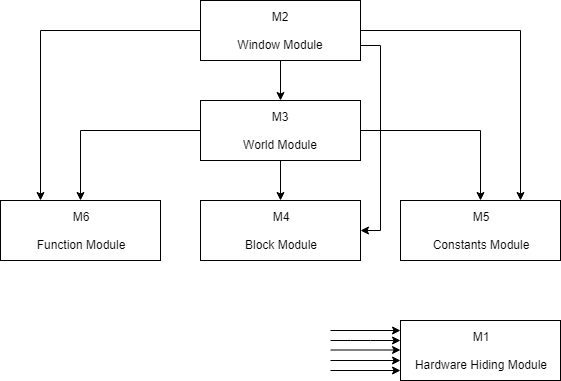
\includegraphics[width=0.7\textwidth]{3XA3ModuleHi.png}
\caption{Use hierarchy among modules}
\label{FigUH}
\end{figure}

%\section*{References}

\bibliographystyle {plainnat}
\bibliography {MG}

\end{document}